\chapter{Topology in non-Hermitian systems}
\label{ch:nh}
In quantum mechanics, the condition that the observable must be a Hermitian operator has a deep physical reasoning - the corresponding expectation value has to be a real-valued number. However, this strong assumption can be relaxed - it is possible to have a non-Hermitian operator with real spectrum. This observation gave rise to the concept of PT-symmetric Hamiltonians, where the real spectrum is guaranteed by the product of parity and time-reversal symmetries~\cite{BenderPT1998}.

Another motivation comes from the open systems. Instead of a full treatment with Lindblad formalism, for instance, nH Hamiltonians can effectively capture the coupling of the system with its environment, where the non-Hermiticity models the gains and losses.

Such system exhibits interesting phenomena without Hermitian counterpart: exceptional points, the skin effect and, as a consequence, the breakdown of bulk-boundary correspondence.

Novel features of nH systems are seen at the level of $2 \times 2$ matrices. Consider a matrix M:
M = \begin{equation}
\begin{pmatrix}
0 & \alpha \\
1 & 0 
\end{pmatrix}
\end{equation}


If $\alpha \neq 1$, $M$ is not diagonalizable, and only admits the Jordan block form. NH matrices have distinct left- and right- eigenvectors. Therefore, a remedy for some problems may be to consider quantities of interests within the biorthogonal quantum mechanics. For instance, the norm is then given by the inner product between left and right eigenvectors. This attempt allowed to restore BB correspondence in some models. Another way is to consider the singular value decomposition (SVD) instead of eigenvalue problem. However, the interpretation of the singular values is not physical (in contrast to the eigendecomposition, where the eigenvalues are the energies)~\cite{SVDHerviou2019}.




In non-Hermitian case, the topology is already manifested in single-band systems (in contrast to Hermitian systems where at least two bands are needed). Also, the winding number for 1D systems is defined through the eigenvalues, not the eigenstates.


\section{Breakdown of bulk-boundary correspondence}


As Hermitian conjugate is not longer equal to complex conjugate and transpose, different type of symmetries appear. Classification, firstly by~\cite{Bernard_2002}, extended recently in Refs.~\cite{PhysRevLett.120.146402, PhysRevX.8.031079, PhysRevB.99.125103}



\section{Exceptional points}
Let us remind the concept of Weyl points. Consider the Hamiltonian in 3D
\begin{equation}
H =\mathbf{k} \cdot \boldsymbol{\sigma} = k_x \sigma_x + k_y \sigma_y + k_z \sigma_z.
\label{eq:weylh}
\end{equation}
This model exhibits a robust generic degeneracy. As all $\sigma_i$ are used, adding other term proportional to $\sigma_i$ only shifts the touching point. Now compare the following model in 2D:
\begin{equation}
H = k_x \sigma_x + k_y \sigma_y + i r \sigma_y
\label{eq:excepth}
\end{equation}
Non-zero $r$ gives rise to  the degeneracies in non-Hermitian band structure called exceptional points. Exceptional points can be seen as equivalents of Weyl nodes as they appear in generic points in $k$-space and one has to get them closer to annhilate them (for example by adding very large mass term).

\begin{figure}
\centering
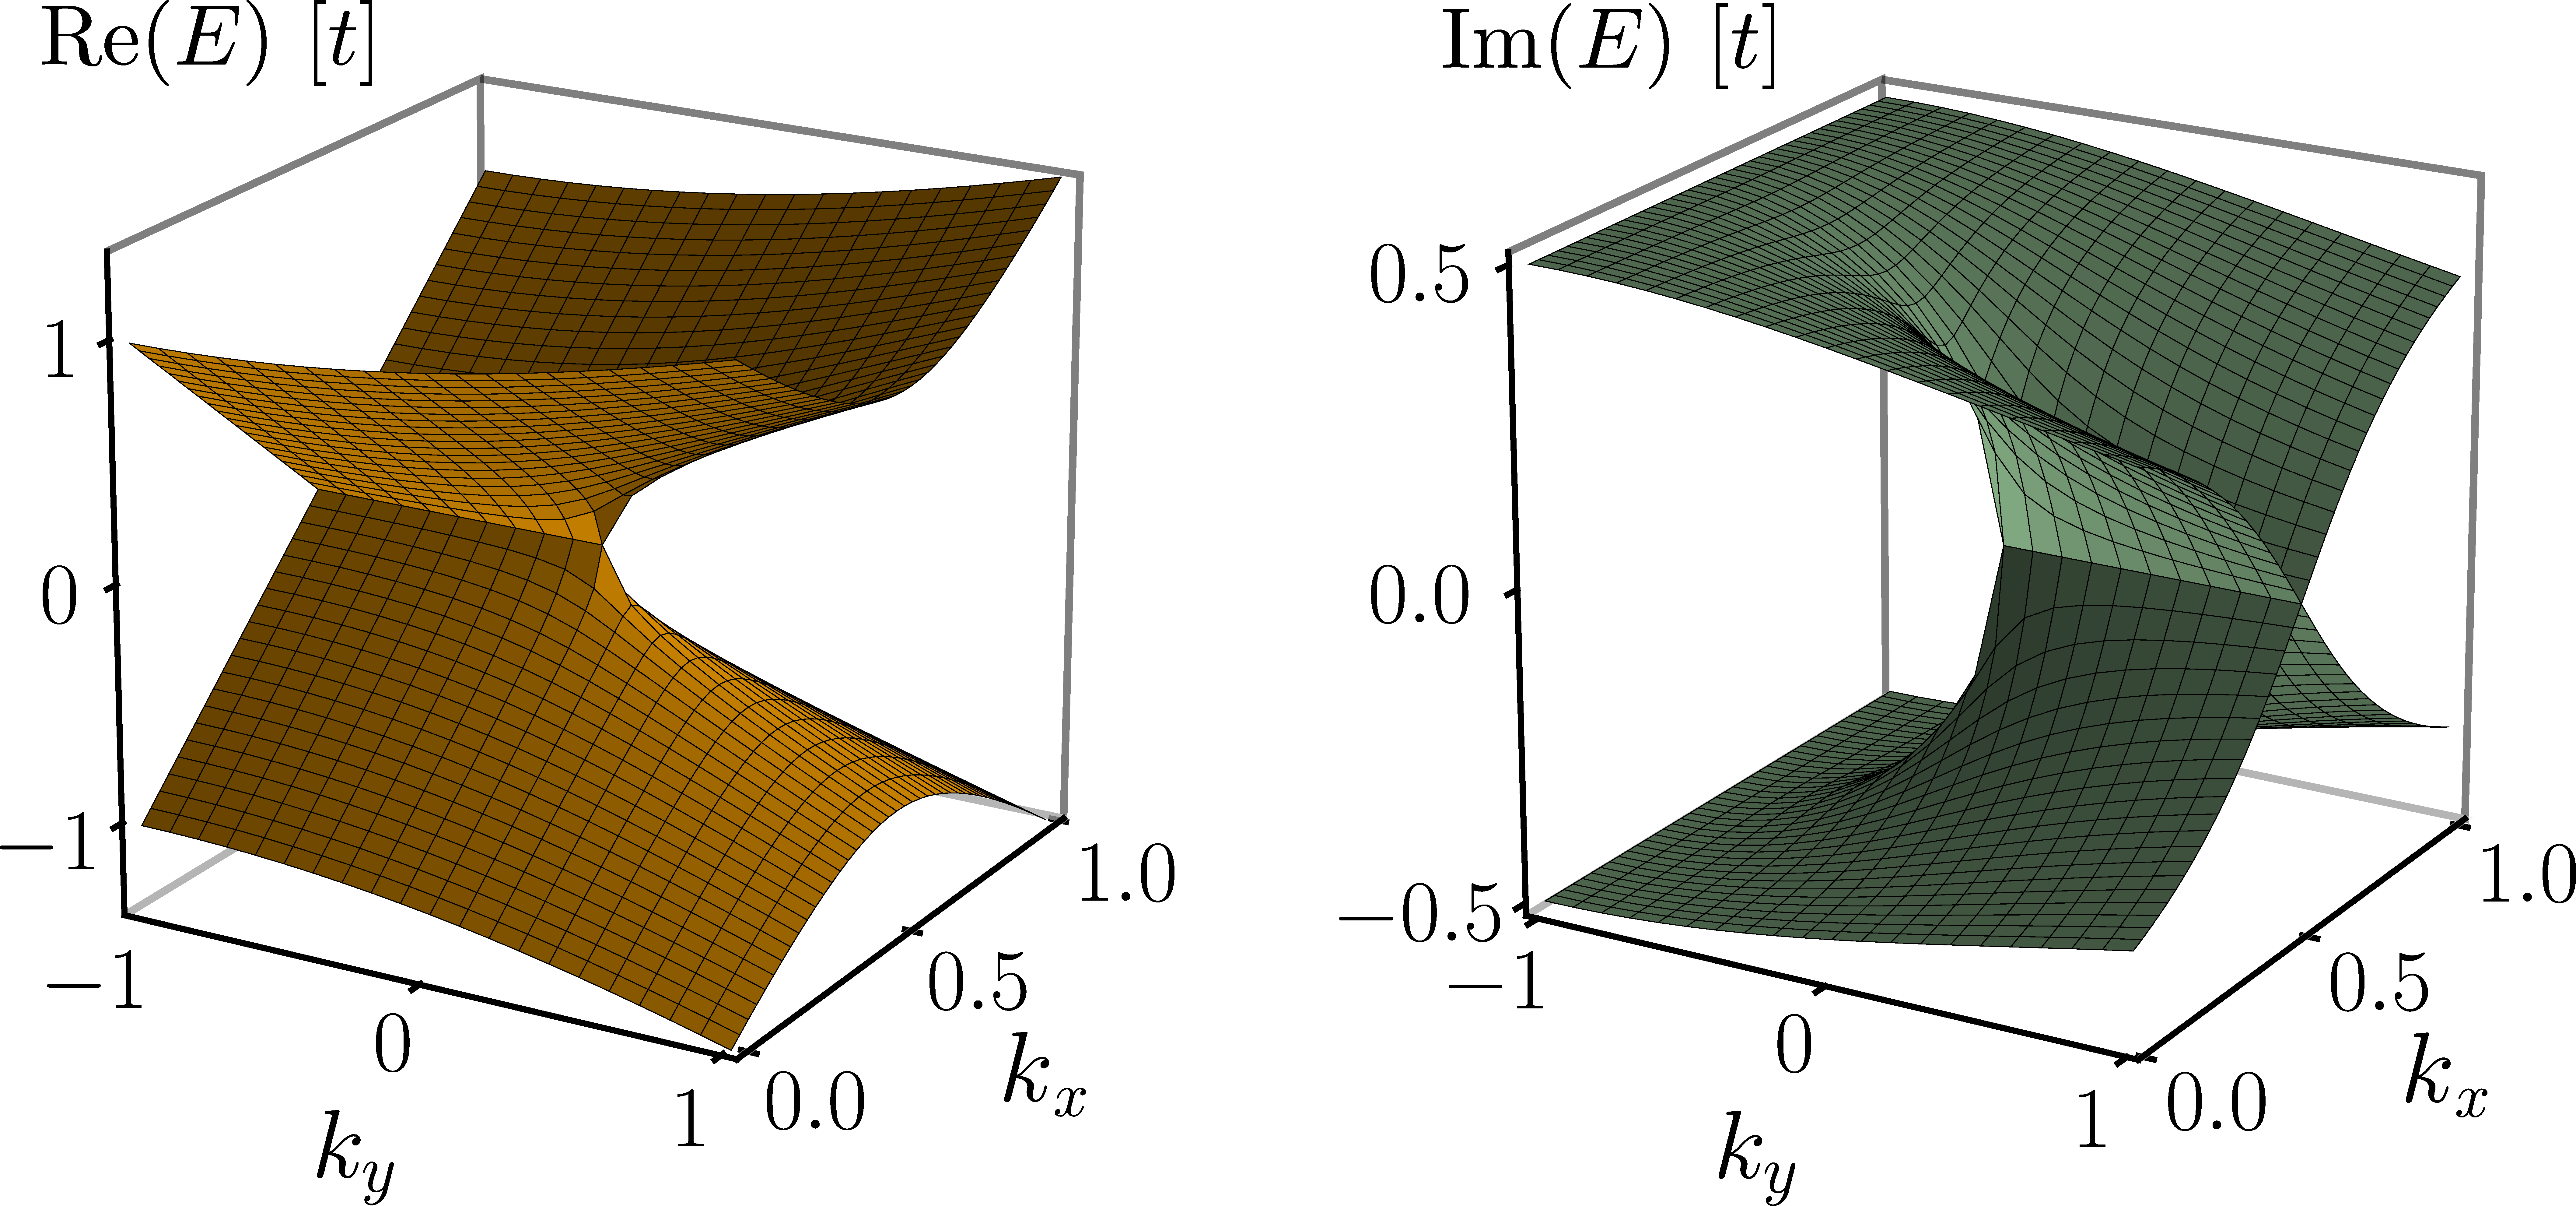
\includegraphics[width=\columnwidth]{nh_exceptional.pdf}
\caption{Real (left) and imaginary (right) part of the spectrum of the Hamiltonian defined by Eq.\eqref{eq:excepth}. Gapless region of real part of the spectrum corresponds to gapped imaginary spectrum and vice versa.}
\label{fig:excepth}
\end{figure}


\subsection{$\pi$-flux model}
To underline the generality of our arguments, we will present the
theory in the language of (non-Hermitian) tight-binding Hamiltonians,
which may represent either a quantum system or the dynamical matrix and response function of a classical system. We start our considerations with the $\pi$-flux tight-binding model on a square lattice. It is characterized by a nearest-neighbor hopping $t$, where exactly one of the four sides of each plaquette has a negative hopping amplitude compared to the three others. These hoppings require a unit cell of two plaquettes of the square lattice [see Fig.~\ref{fig: 1}~a)]. The Bloch Hamiltonian for a system with periodic boundary conditions (PBC) in $x$ and $y$ directions, yielding the momenta $k_x$ and $k_y$, can be written as
\begin{equation}
H_{\mathrm{\pi}}(k_x,k_y)=
t\begin{pmatrix}
2\cos\,k_y&1+e^{-ik_x}\\
1+e^{ik_x}&-2\cos\,k_y
\end{pmatrix}.
\label{eq: pi flux}
\end{equation}
The model has two Dirac-like band touchings at momenta $(k_x,k_y)=(\pi,\pi/2)$ and $(k_x,k_y)=(\pi,3\pi/2)$ [see Fig.~\ref{fig: 1}~a) for the band structure].

We add a non-Hermitian (gain/loss) term as a diagonal hopping through
one of the plaquettes in the unit cell [see Fig.~\ref{fig: 1}~a)]. It
assigns a complex amplitude $i r$ (with $r$ a real number) to
the the process of a particle hopping along the diagonal toward the
upper right, and the exact same amplitude $i r$ to the
reversed process. Hermiticity would require that the latter
process has the complex conjugated amplitude $-i r$. As such, the addition 
\begin{equation}
H(k_x,k_y)=
H_{\mathrm{\pi}}(k_x,k_y)
-ir \begin{pmatrix}
0&e^{ik_y}\\
e^{-ik_y}&0
\end{pmatrix}
\label{eq: non-Hermitian H}
\end{equation}
violates Hermiticity for this diagonal hopping process.
Despite its non-Hermiticitiy, the model still is reciprocal, as it satisfies
$H(k_x,k_y)=H^{\mathsf{T}}(-k_x,-k_y)$ under transposition. 

Hamiltonian~\eqref{eq: non-Hermitian H} has two complex-valued eigenbands with remarkable properties: they  touch (\ie the two eigenvalues have equal real and imaginary part) in two pairs of points. Upon introducing a finite $r$, the Dirac points of the original $\pi$-flux model each split into a pair of these points. Such degeneracy points in non-Hermitian systems are called exceptional points and are the generic band touchings in a space with two parameters (here, $k_x$ and $k_y$). The band structure in the vicinity of an exceptional point is illustrated in Fig.~\ref{fig: 1}~b).

We proceed to consider Hamiltonian~\eqref{eq: non-Hermitian H} with OBC in $x$-direction, which leaves $k_y \in [0,2\pi]$ well defined as a boundary momentum, and define $\tilde{H}(k_y)$ as the Hamiltonian for the strip geometry. While $\tilde{H}^\top(k_y) = \tilde{H}(-k_y)$ guarantees reciprocity of the full system, each instance of $\tilde{H}(k_y)$ \textit{locally} breaks reciprocity for a fixed $k_y$ when seen as a purely one-dimensional model, except for $k_y = - k_y \mod(2\pi)$. The effective 1D model for a given $k_y$ exhibits the non-Hermitian skin effect as discussed in Refs.~\cite{Shunyu2018prl,song2019non}: The eigenstates of a Hermitian system form an orthonormal basis whose squared amplitudes, when summed over all states, are equal on all lattice sites. In a non-Hermitian system this need not be the case, since right (left) eigenstates of a non-Hermitian matrix do not individually form an orthonormal basis. As a result, they can all be localized at only one edge of the system, which defines the skin effect. In our model, the skin effect is realized due to the term proportional to $r$ in Eq.~\eqref{eq: non-Hermitian H}, which renders the hopping probability for going right different from the probability for going left. This leads to an accumulation of \emph{all eigenstates} towards only one edge.


\begin{figure*}[t]
\begin{center}
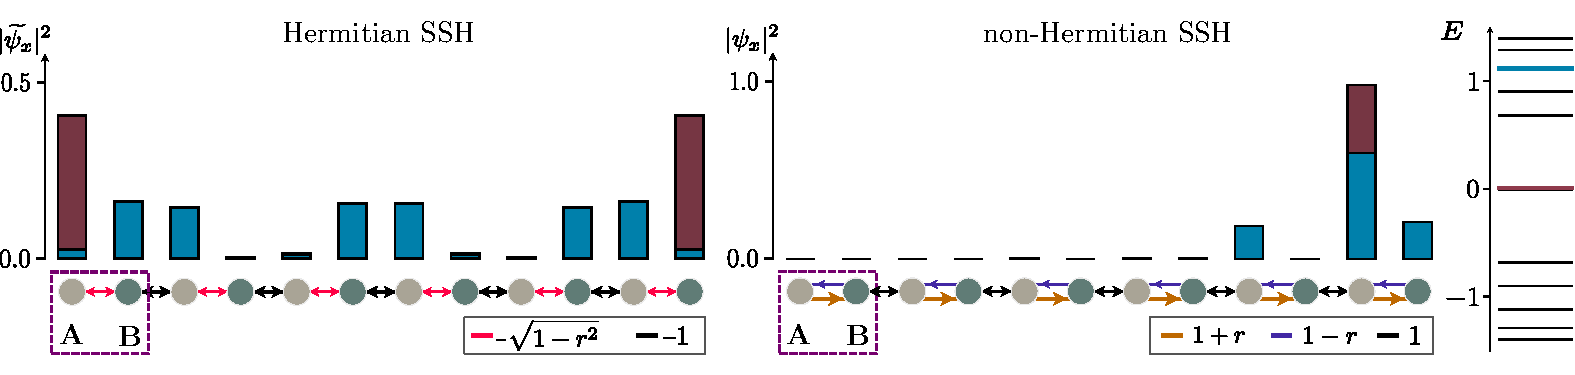
\includegraphics[width=1\textwidth]{SI-SSH.pdf}
\caption{
Relation between the Hermitian ($r = 0$) and non-Hermitian ($r = 0.9$) dimerized chain, the SSH model. The spectrum of both models is equal with open boundary conditions, including SSH-type end states. However, \emph{all} states in the non-Hermitian model are localized on one side of the system. 
The amplitude at each lattice site for the two eigenstates marked in the spectrum on the right are plotted with the respective color.
}
\label{fig: nonunitarytransform}
\end{center}
\end{figure*}

We expand the Hamiltonian~(2) to linear order in the momentum deviations $\delta k_y$ around these two points and in $r$ [\ie we drop a term $\mathcal{O}(r\,\delta k_y)$]. 
Denote by 
$H^{(\pm)}_{x\alpha,x'\alpha'}(\delta k_y)$ the matrix elements for the thus expanded strip Hamiltonian,
where $x,x'=1,\cdots, L$ labels the unit cell across the strip and $\alpha,\alpha'\in\{1,2\}$ refers to the two sublattices. 
We will now show that, under OBCs but \emph{not} PBCs, this non-Hermitian Hamiltonian is related, by \emph{non-unitary} transformations, to a pair of well-known Hermitian Hamiltonians. Our discussion closely follows Ref.~\cite{Shunyu2018prl}. The transformation (setting $t=1$)
\begin{equation}
O_{x,x'}^{(\pm)}=\delta_{x,x'}\left(\sqrt{\frac{1\mp r}{1\pm r}}\right)^x M^{(\pm)}(r),
\end{equation}
with $M^{(\pm)}(r)$ an appropriate $2\times2 $ nonsingular matrix acting on the sublattice space,
maps  $\tilde{H}^{(\pm)}(\delta k_y)=\left(O^{(\pm)}\right)^{-1}H^{(\pm)}(\delta k_y)O^{(\pm)}$, with
\begin{equation}
\begin{split}
\tilde{H}^{(\pm)}_{x,x'}(\delta k_y)
=&\,
\delta_{x,x'}
\begin{pmatrix}
2\delta k_y&-\sqrt{1-r^2}\\
-\sqrt{1-r^2}&-2\delta k_y
\end{pmatrix}
\\
&\,
-
\begin{pmatrix}
0&\delta_{x',x+1}\\
\delta_{x',x-1}&0
\end{pmatrix}.
\end{split}
\label{eq: SSH Hamiltonian}
\end{equation}

For $\delta k_y=0$, Eq.~\eqref{eq: SSH Hamiltonian} is the tight-binding Hamiltonian for a dimerized chain, known as the Su-Schrieffer-Heeger model  [see Fig.~\ref{fig: nonunitarytransform})]. For $-1<r<1$, $r\neq0$, the chain is bulk insulating but has one SSH-type midgap state localized at each end of the chain. Its bulk states are of delocalized Bloch character, while the end states are exponentially localized with a ratio $\tilde{\psi}_{x,\alpha}/\tilde{\psi}_{x\pm1,\alpha}=\sqrt{1-r^2}$ of wave function amplitudes on neighboring lattice sites. [We denote by by $\psi_{x,\alpha}(\delta k_y)$ and $\tilde{\psi}_{x,\alpha}(\delta{k_y})$ the eigenstates of $H^{(\pm)}(\delta k_y)$ and $\tilde{H}^{(\pm)}(\delta k_y)$, respectively.]
Finite but small $\delta k_y$ mainly has the effect of lifting the degeneracy of the SSH-type end states from eigenvalue 0 to $\pm 2\delta k_y$. 

Being related by $O^{(\pm)}$, $\tilde{H}^{(\pm)}(\delta k_y)$ and the non-Hermitian Hamiltonian $H^{(\pm)}(\delta k_y)$ are isospectral, but their eigenstates differ in important ways. The $x$-dependent factor in $O^{(\pm)}$ turns \emph{all} the Bloch-type bulk states into exponentially localized states, with $\psi_{x,\alpha}/\psi_{x\pm1,\alpha}\approx \sqrt{2/(1\pm r)-1}$ -- which is a stronger exponential decay than that of the SSH-type end states. Whether the localization is on the left or right edge of the system depends on the sign of $r$ and is opposite for $H^{(+)}(\delta k_y)$ and $H^{(-)}(\delta k_y)$. We conclude that on a strip geometry all eigenmodes of the model Eq.~(2) are localized on one side of the sample for $k_y \sim \pi/2$ and on the opposite side for $k_y \sim 3\pi/2$.
This constitutes the \emph{reciprocal skin effect}, enabled by the non-Hermiticity of the Hamiltonian. Reciprocity enforces the opposite localization at opposite momenta $k_y$.

\section{Skin effect}
nH Hamiltonians are sensitive to the boundary conditions. Eigenstates localization properties may change dramatically. All states for the system in an open geometry may be exponentially localized on the one edge, which is dubbed the skin effect (note: this has nothing in common with a typical skin effect, where the electrons in a conductor prefer to flow far from the middle due to electron-electron repulsion).

Previously, it was known that the skin effect can be induced by having unbalanced directed hoppings. However, this breaks the reciprocity, defined as 
\begin{equation}
H (k) = H^{T} (-k)
\label{eq:recipSE}
\end{equation}


\subsection{Reciprocal skin effect}

Here, we show that in two- or higher-dimensions it is possible to have the skin effect with the condition defined by Eq.~\eqref{eq:recipSE}.

